\documentclass[tikz, border=3mm]{standalone}
\usepackage{tikz}

\begin{document}
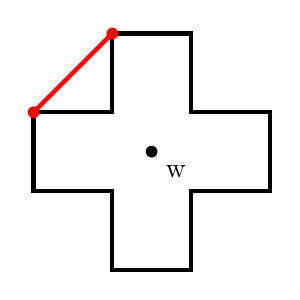
\begin{tikzpicture}[
    dot/.style={fill=red, circle, inner sep=1.5pt}, % Style for red dots
        black_dot/.style={fill=black, circle, inner sep=1.5pt} % Style for black dots
]
% Define coordinates for the vertices (adjust size/proportions as needed)
\coordinate (p1) at (0.5, 0.5);
\coordinate (p2) at (0.5, 1.5);
\coordinate (p3) at (-0.5, 1.5);
\coordinate (p4) at (-0.5, 0.5);
\coordinate (p5) at (-1.5, 0.5);
\coordinate (p6) at (-1.5, -0.5);
\coordinate (p7) at (-0.5, -0.5);
\coordinate (p8) at (-0.5, -1.5);
\coordinate (p9) at (0.5, -1.5);
\coordinate (p10) at (0.5, -0.5);
\coordinate (p11) at (1.5, -0.5);
\coordinate (p12) at (1.5, 0.5);
    \coordinate (O) at (0,0);


% Draw the plus-sign shape by connecting the vertices
% Use 'ultra thick' to match the image style
\draw[black, ultra thick]
    (p1) -- (p2) -- (p3) -- (p4) -- (p5) -- (p6) -- (p7) -- (p8) -- (p9) -- (p10) -- (p11) -- (p12) -- cycle;

\draw[red, ultra thick] (p5) -- (p3);

%\draw[red, ultra thick] (p5) -- (p3);

%\node[dot, black, inner sep=0.1pt] at (0,0) {w};

    \node[black_dot, label={[black]below right:w}] at (O) {};


    % Add red point indicators at p5 and p3 (drawn last to be on top)
    \node[dot] at (p5) {};
    \node[dot] at (p3) {};
% Alternative using plot coordinates (more compact)
% \draw[black, ultra thick] plot coordinates {
%     (0.5, 0.5) (0.5, 1.5) (-0.5, 1.5) (-0.5, 0.5) (-1.5, 0.5)
%     (-1.5, -0.5) (-0.5, -0.5) (-0.5, -1.5) (0.5, -1.5) (0.5, -0.5)
%     (1.5, -0.5) (1.5, 0.5)
% } -- cycle;

\end{tikzpicture}
\end{document}